%%
%  ******************************************************************************
%  * #file    Szablon_raportu_EN_Latex.tex
%  * #author  Adrian Wójcik   adrian.wojcik(at)put.poznan.pl
%  *          
%  * #commit  Patryk Kościk   koscikpatryk(at)gmail.com
%  *          Modified the template for Projekt przejsciowy purposes          
%  *          
%  * #version 1.0
%  * #date    09-Mar-2022
%  * #brief   PROJPRZEJ
%  *
%  ******************************************************************************
%%  
\documentclass[11pt, a4paper]{article}

\usepackage{SM_template}

% Wypełnijcie te dyrektywy zgodnie z waszym tematem
% \lab      -> NAZWA CZUJNIKA, np.: 'DHT22'
% \comment  -> Króciutki opis co to, np.: 'Cyfrowy budżetowy czujnik temperatury'
%

\lab{Moduł KY-013}
\comment{Analogowy czujnik temperatury otoczenia}
\author{Antoni Borowski}
\addbibresource{bib/KY-013.bib}

% Absolutny zakaz dotykania tego tutaj bo jak dotkiecie to coś jebnie
\university{Politechnika Poznańska}
\faculty{Wydział Automatyki, Robotyki i Elektrotechniki}
\institute{Instytut Robotyki i Inteligencji Maszynowej}
\department{Zakład Sterowania i Elektroniki Przemysłowej}

\nocite{*}


%%
%
% Początek dokumentu
%
%%
\begin{document}

%% Strona tytułowa %%
\mainpage{{KY-013/foto}}
\newpage

\section*{Opis elementu} \addcontentsline{toc}{section}{Wstęp}
 Termistor jest rezystorem półprzewodnikowym o rezystancji silnie zależnej od temperatury (w dużo większym stopniu niż w przypadku standardowych oporników). Rezystancja zmienia się w zależności od temperatury otoczenia. Termistor NTC płynnie zmniejsza rezystancję między swoimi wyprowadzeniami, kiedy temperatura otoczenia rośnie. Jest to możliwe dzięki zjawisku generacji termicznej, czyli samoistnemu rozpadaniu się wiązań między atomami budujących strukturę krystaliczną pod wpływem temperatury. Powstaje wtedy para elektron-dziura, swobodne nośniki prądu elektrycznego. Wartość zmiany rezystancji zależy od rodzaju materiału użytego w termistorze. Związek między temperaturą i rezystancją termistora jest nielinearny. Typowy wykres termistora pokazano na rysunku Rys.1(b).
\vspace{0.5cm}
\begin{figure}[h!]
\centering
\begin{subfigure}{.5\textwidth}
  \centering
  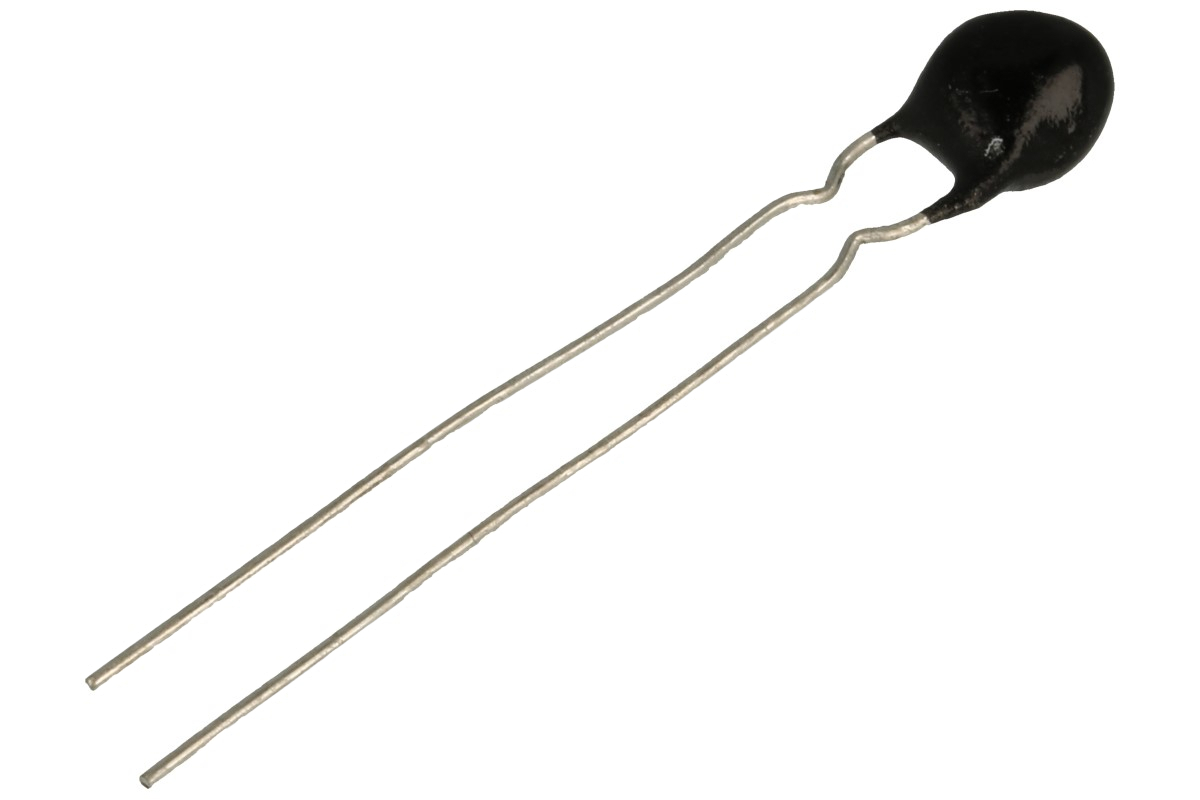
\includegraphics[width=.94\linewidth]{fig/KY-013/zdj_modułu/fig2.jpg}
  \caption{Termistor \cite{ArduinoModules:grab}}
  \label{fig:sub1}
\end{subfigure}%
\begin{subfigure}{.5\textwidth}
  \centering
  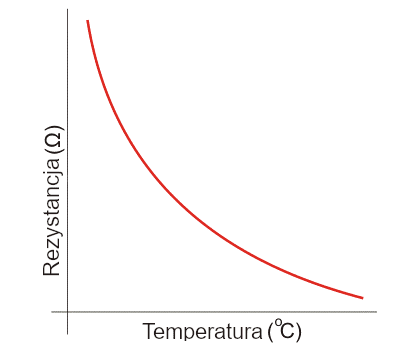
\includegraphics[width=0.7\linewidth]{fig/KY-013/zasada_dzialania/wykress.png}
  \caption{Związek między temperaturą i rezystancją \cite{bot:wykres}}
  \label{fig:sub2}
\end{subfigure}
\caption{Wygląd termistora oraz charakterystyka}
\label{fig:test}
\end{figure}
\newline
Czujnik KY-013 składa się z termistora NTC, wbudowanego rezystora 10k $\Omega$ oraz trzech pinów męskich.


\begin{figure}[h!]
\centering
\begin{subfigure}{.5\textwidth}
  \centering
  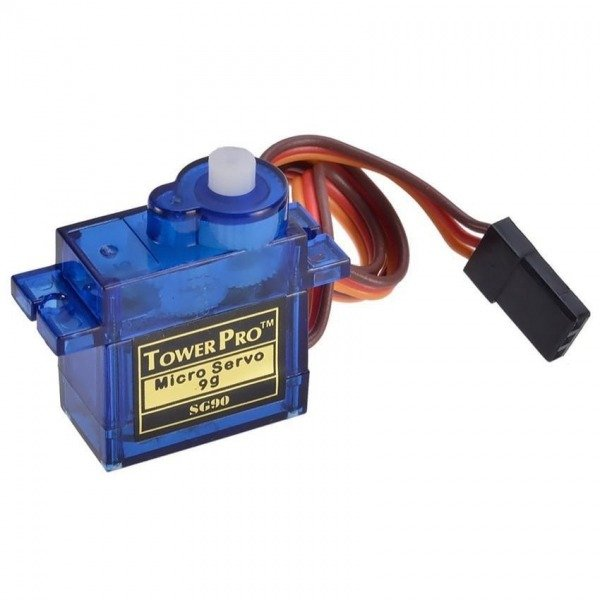
\includegraphics[width=.45\linewidth]{fig/KY-013/zdj_modułu/fig1.png}
  \caption{Moduł KY-013 \cite{ArduinoModules:Switch}}
  \label{fig:sub1}
\end{subfigure}%
\begin{subfigure}{.5\textwidth}
  \centering
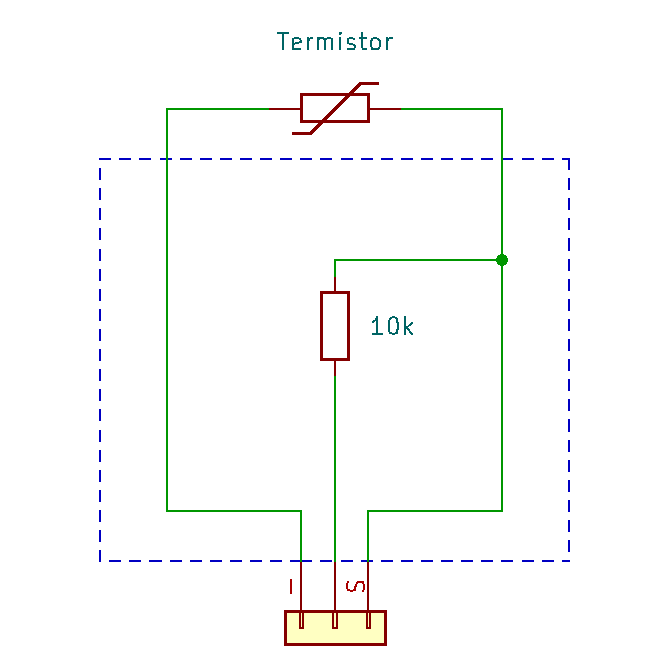
\includegraphics[width=.81\linewidth]{fig/KY-013/zasada_dzialania/schemacik.png}
\caption{Schemat modułu}
  \label{fig:sub2}
\end{subfigure}
\caption{Wygląd modułu oraz jego schemat}
\label{fig:test}
\end{figure}

\newpage
\section*{Użycie czujnika}
Te czujniki temperatury działają jako element pasywny w obwodzie. Są precyzyjnym, tanim i wytrzymałym narzędziem do pomiaru temperatury. Chociaż nie działają dobrze w ekstremalnie wysokich lub niskich temperaturach, to wciąż posiadają wiele różnych zastosowań. Idealnie nadają się, gdy wymagany jest precyzyjny odczyt temperatury. Są powszechnie stosowane do pomiaru temperatury cieczy i powietrza otoczenia jako termometry termistorowe. Zastosowanie termistorów możliwe najczęściej jest w termostatach czy innych urządzeniach domowego użytku, jak piekarniki i lodówki.
\vspace{0.5cm}

Poniżej przedstawiono zmianę rezystancji przy wykorzystaniu źródła ciepła - ognia oraz wykonano pomiar multimetrem. 
\begin{figure}[h!]
\begin{subfigure}{.5\textwidth}
  \centering
  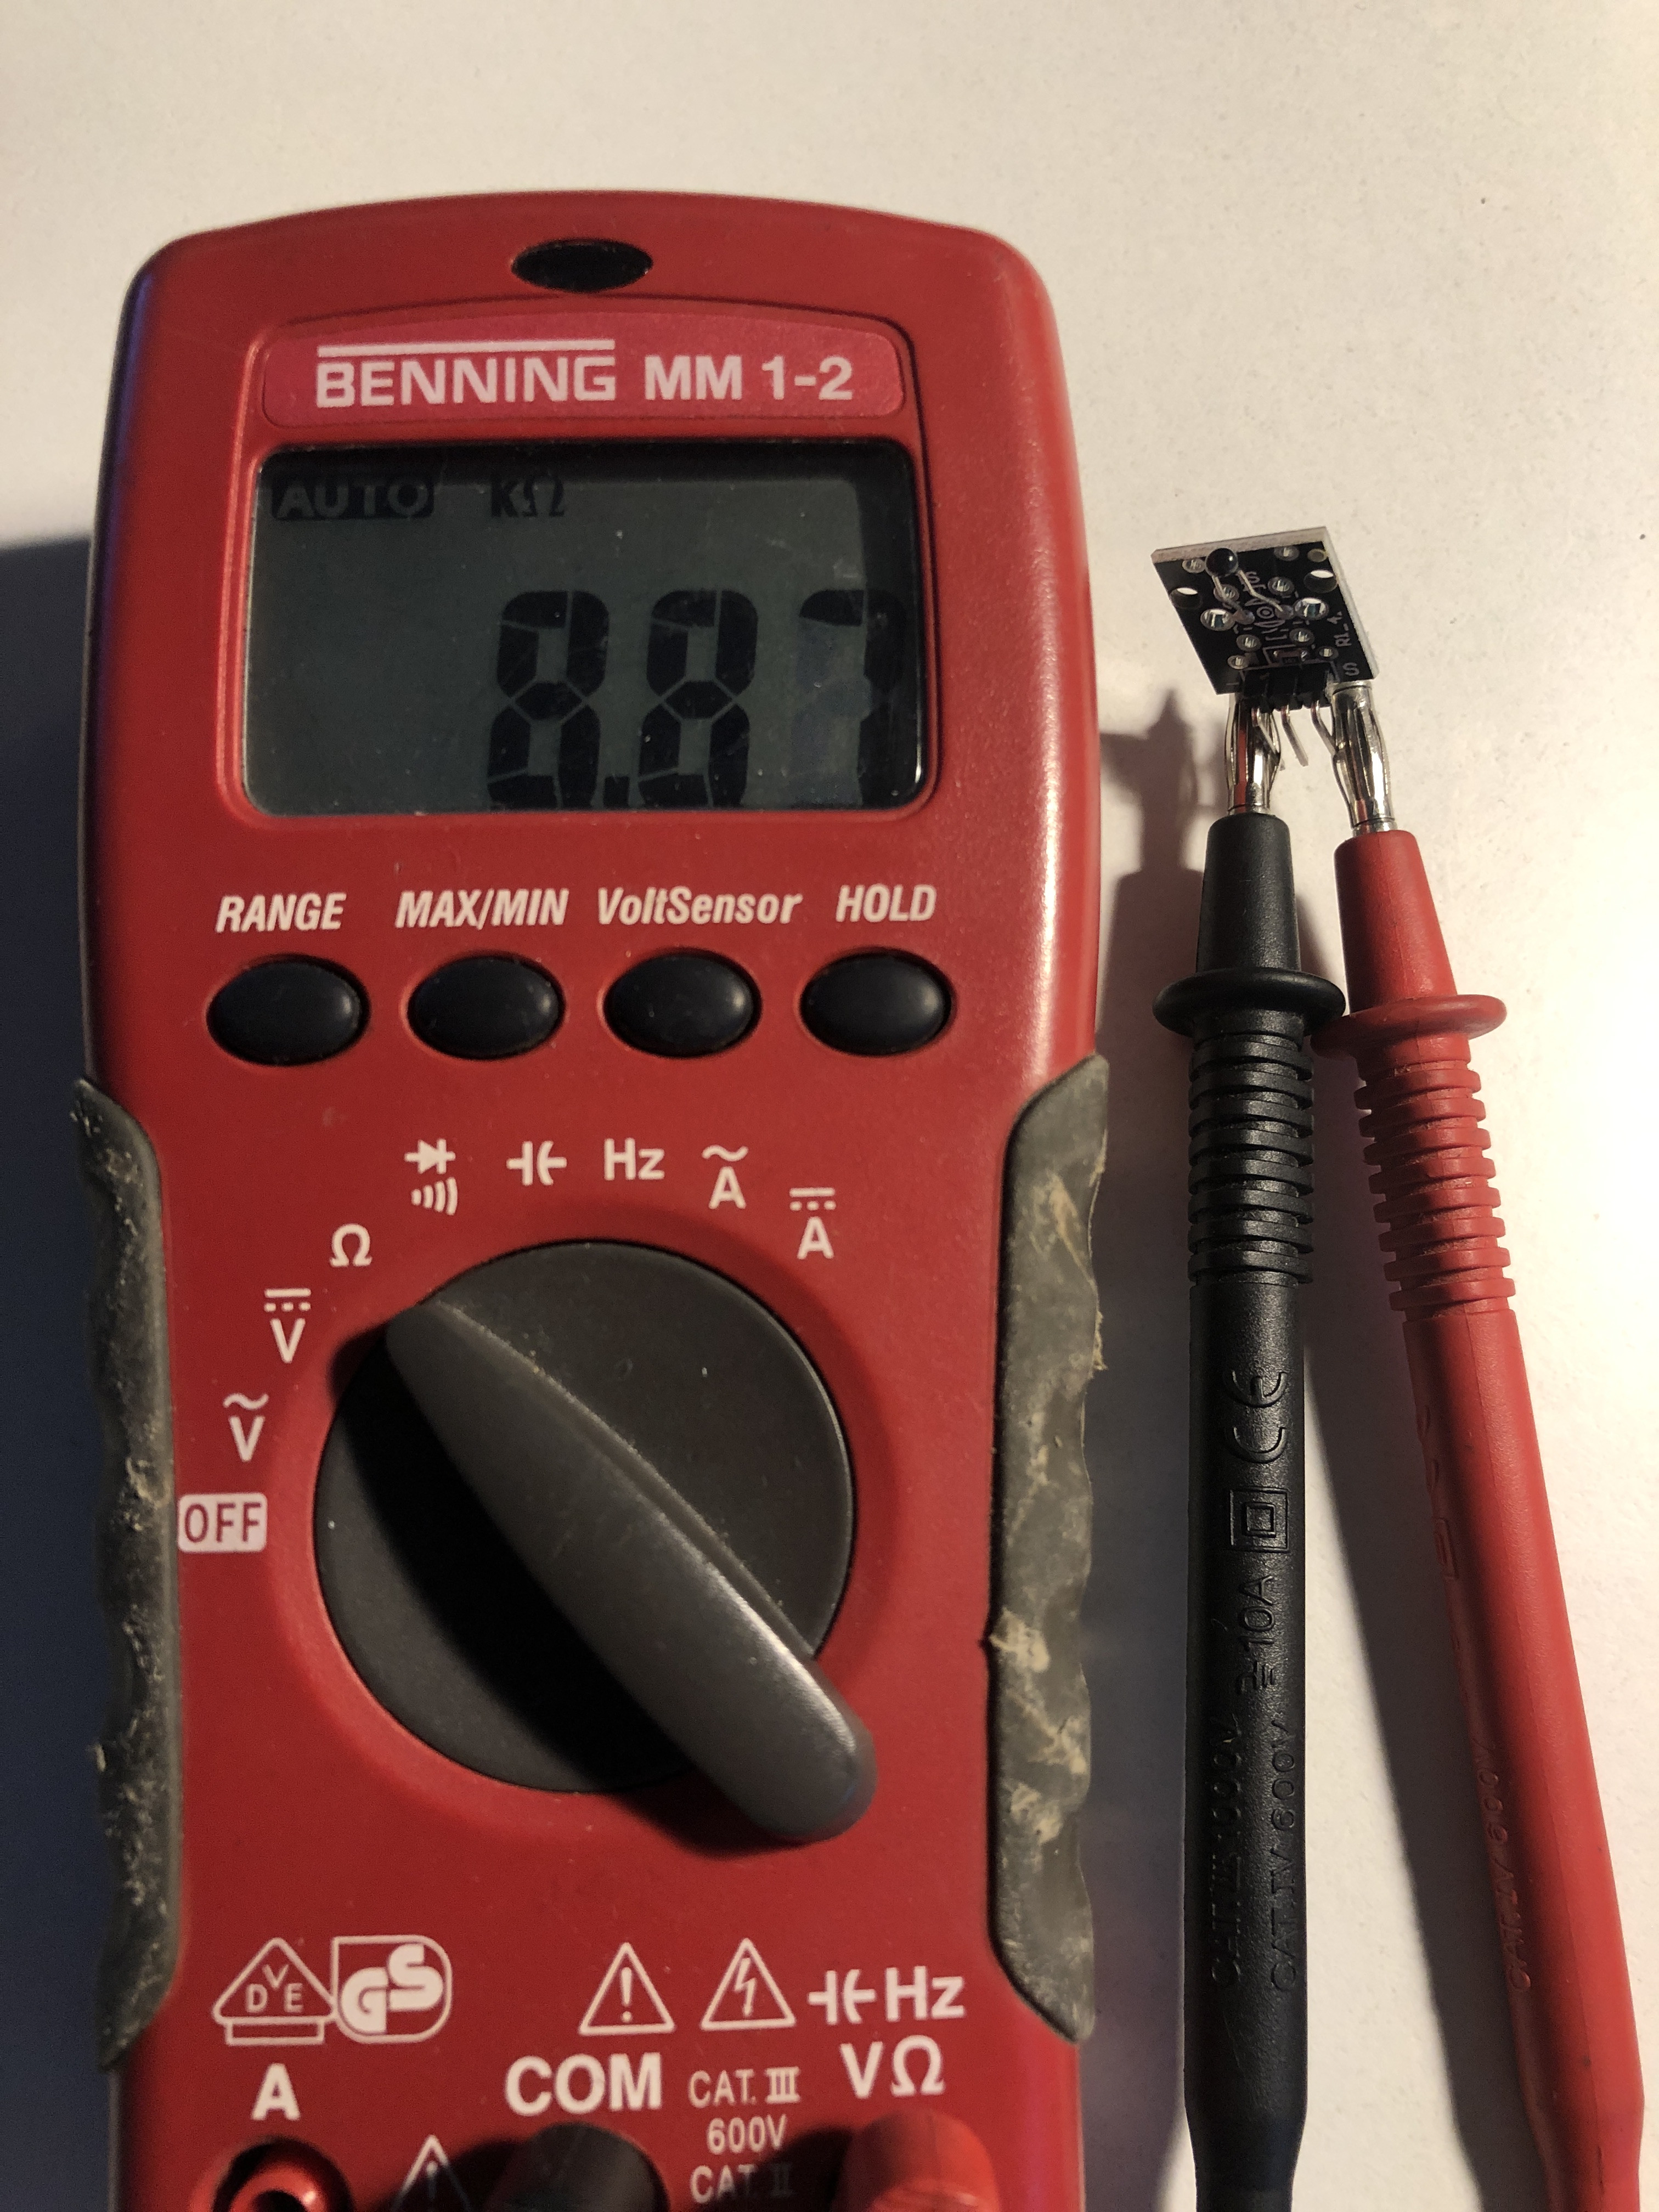
\includegraphics[width=.7\linewidth]{fig/KY-013/działanie_ukladu/1.jpg}
  \caption{Temperatura pokojowa - rezystancja 8.87k $\Omega$}
  \label{fig:sub1}
\end{subfigure}%
\begin{subfigure}{.5\textwidth}
  \centering
  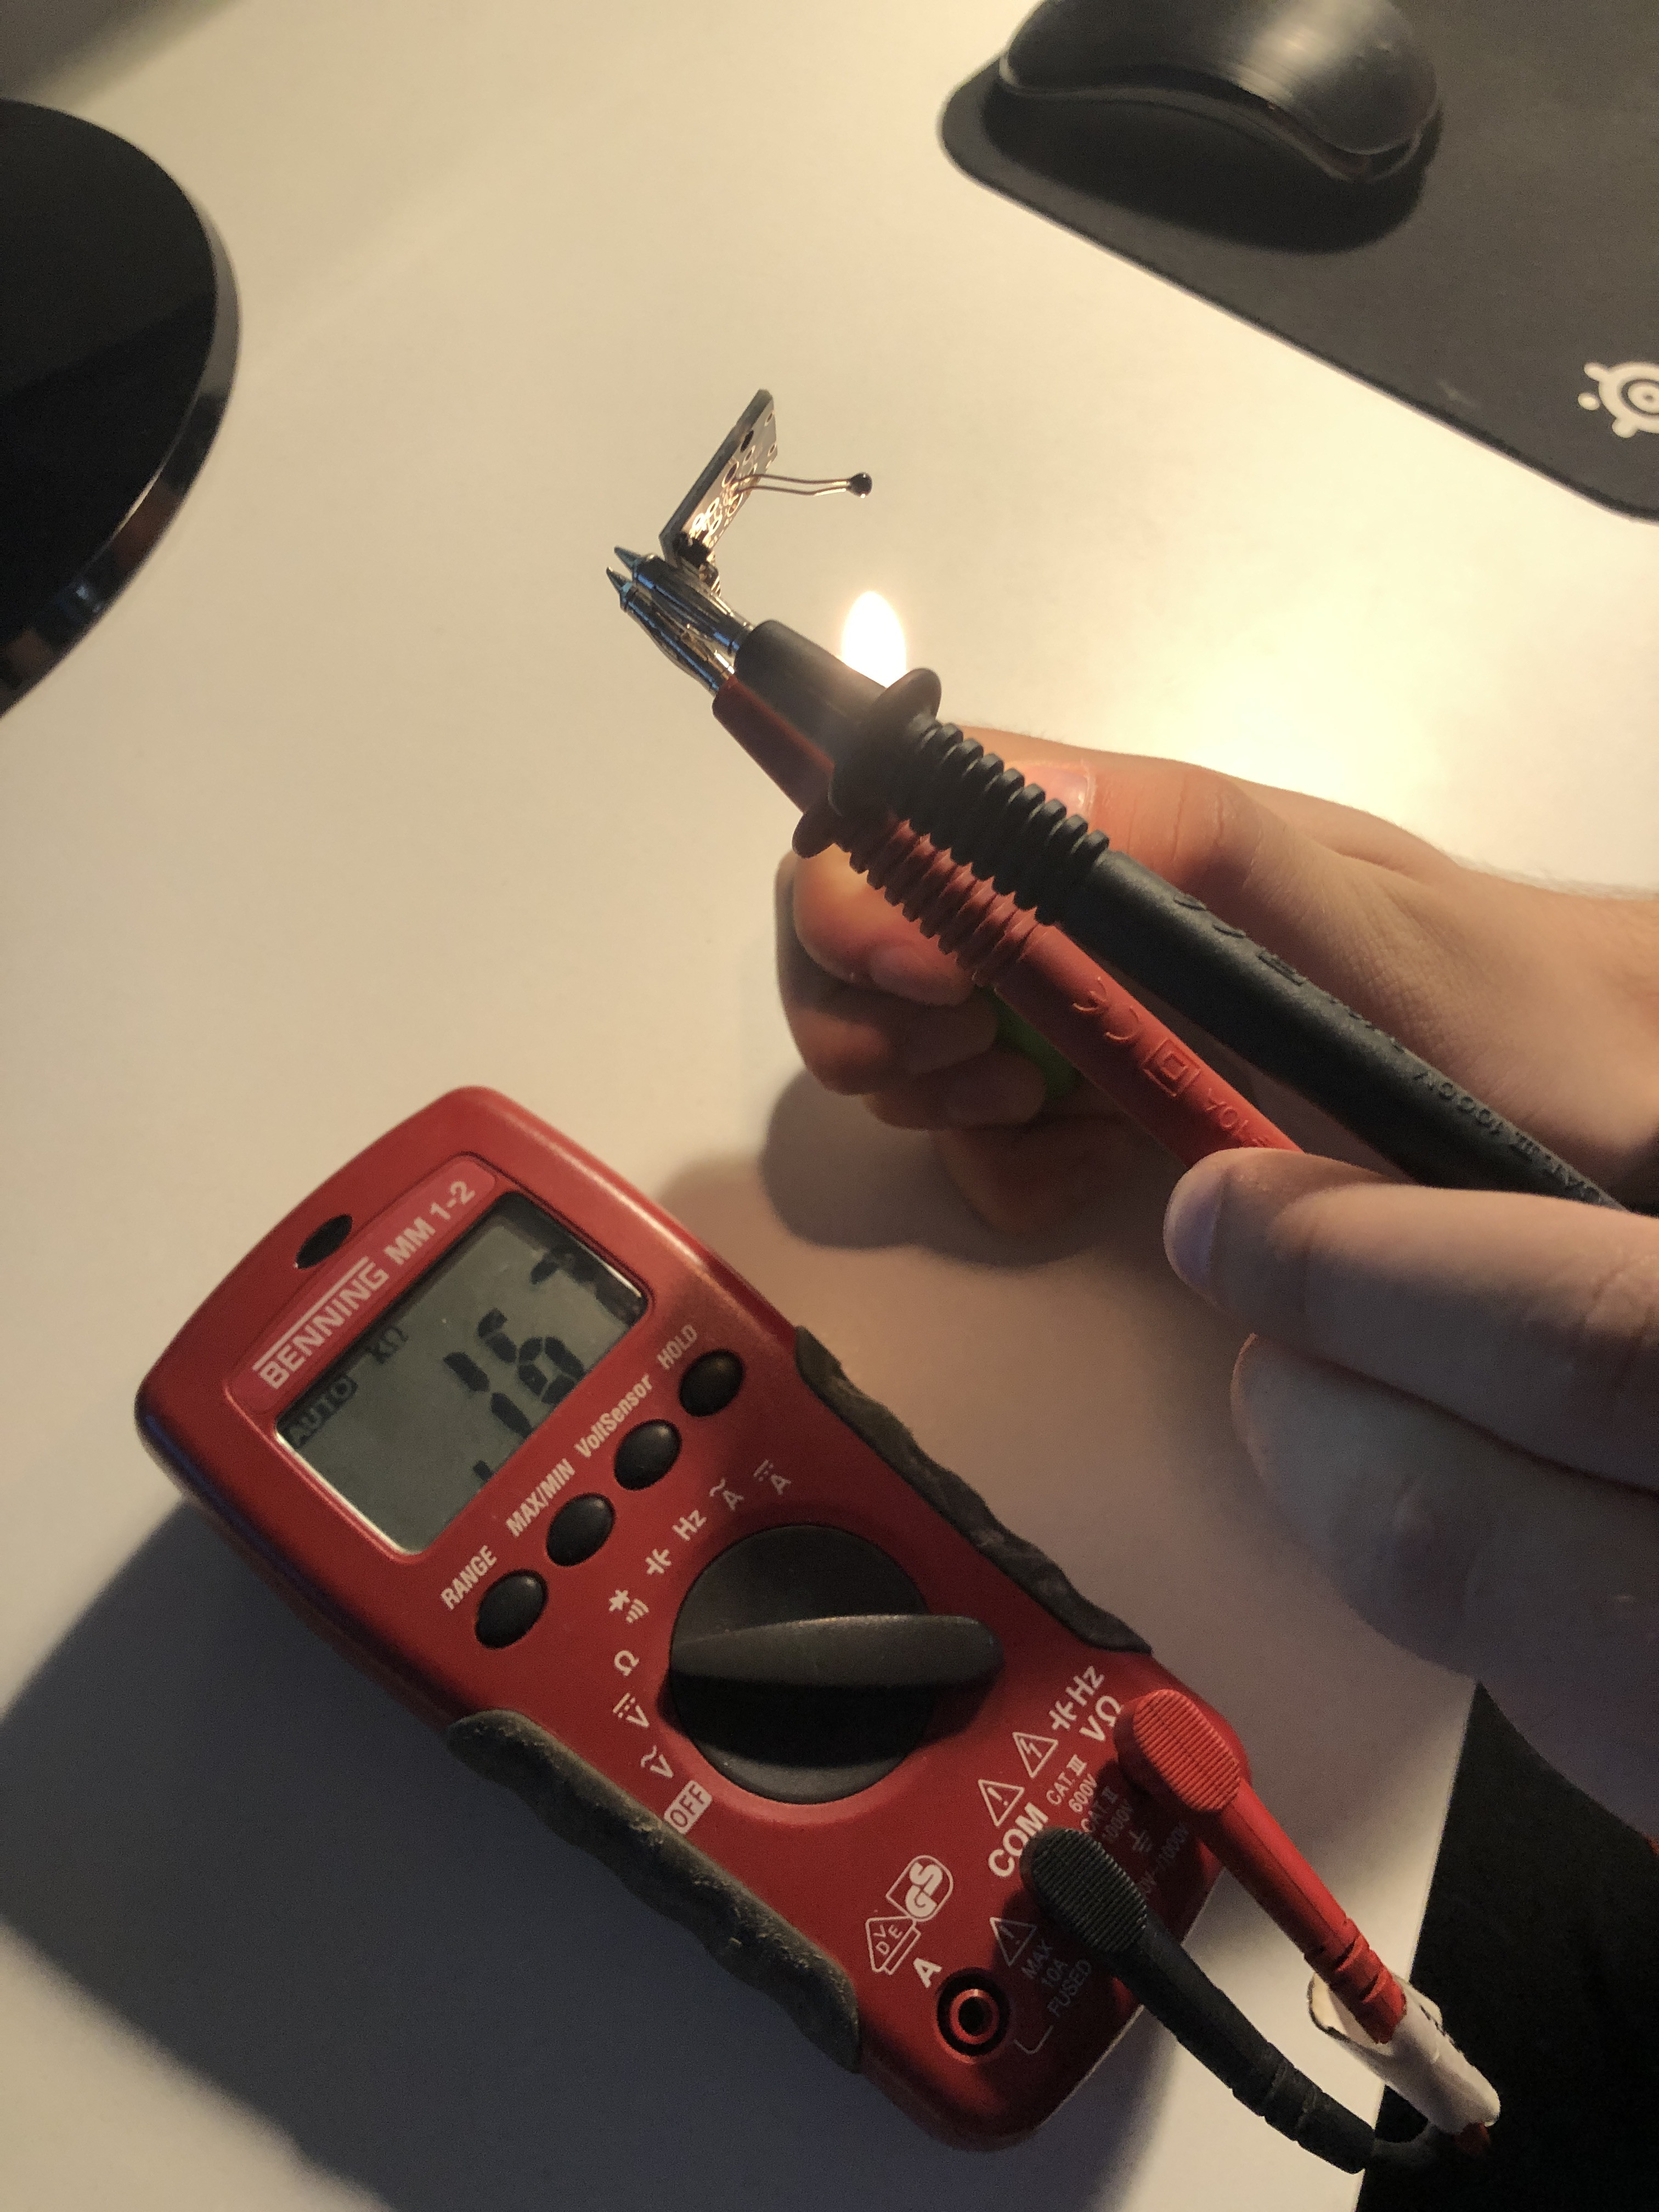
\includegraphics[width=0.7\linewidth]{fig/KY-013/działanie_ukladu/2.jpg}
  \caption{Podgrzanie powietrza - rezystancja 167 $\Omega$}
  \label{fig:sub2}
\end{subfigure}
\caption{Zmiana rezystancji modułu pod wpływem ciepła}
\label{fig:test}
\end{figure}

\vspace{0.5cm}
\begin{figure}[h!]
    \centering
    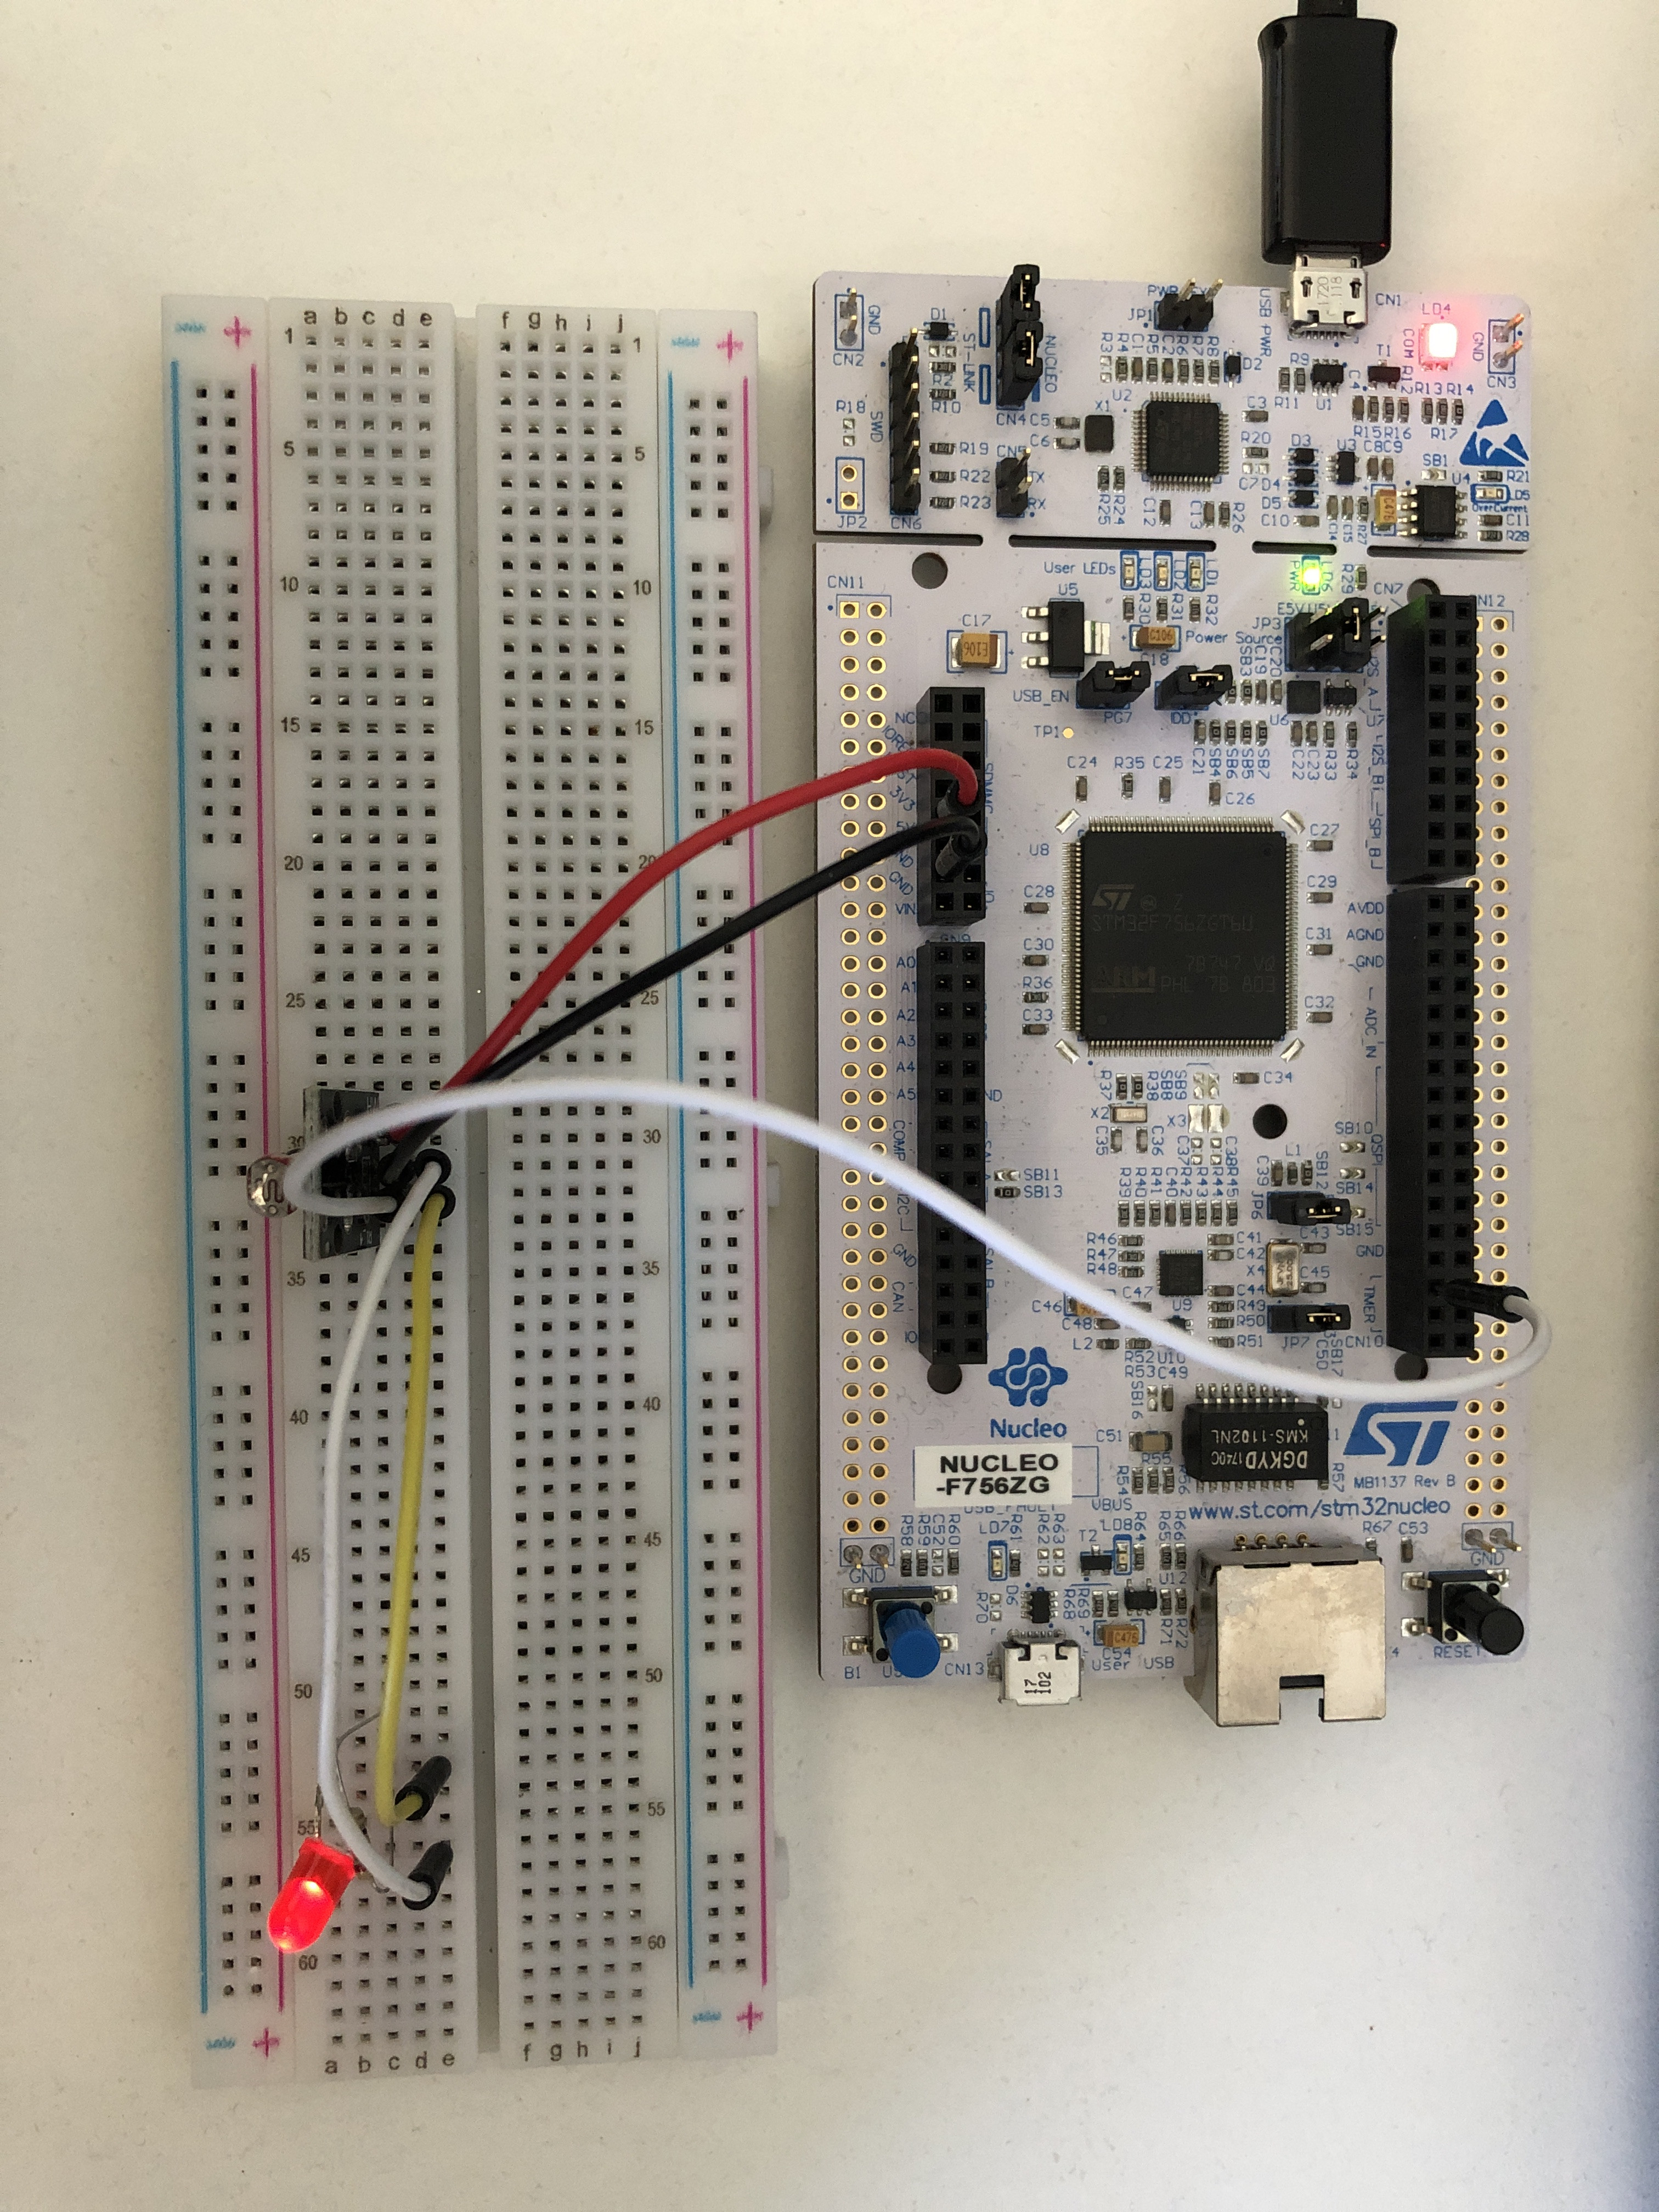
\includegraphics[width=0.4\textwidth,angle=90]{fig/KY-013/działanie_ukladu/final.jpg}
    \caption{Podłączenie modułu}
    \label{fig:my_label}
\end{figure}
\newpage 

Zależność między rezystancją a temperaturą w termistorze NTC określa poniższe równanie:
$$R_{T}=R_{0}e^{\beta(\frac{1}{T}-\frac{1}{T_0})}$$
gdzie:
\begin{itemize}
    \item $R_T$ - rezystancja przy temepraturze $T$ (K)
    \item $R_0$ - rezystancja przy temperaturze $T_0$ (K)
    \item $T_0$ - tempertura odniesienia (około 25$^\circ$C)
    \item $\beta$ stała, której wartość zależy od właściwości materiału - nominalnie przyjmuje się 4000.
\end{itemize}
\begin{figure}[h!]
\begin{subfigure}{.5\textwidth}
  \centering
  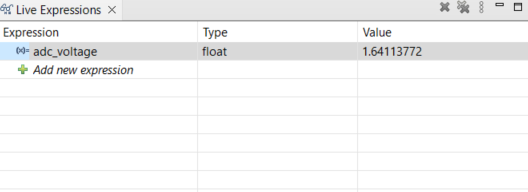
\includegraphics[width=1\linewidth]{fig/KY-013/działanie_ukladu/pokoj.png}
  \caption{Napęcie uzyskane w temperaturze pokojowej}
  \label{fig:sub1}
\end{subfigure}%
\begin{subfigure}{.5\textwidth}
  \centering
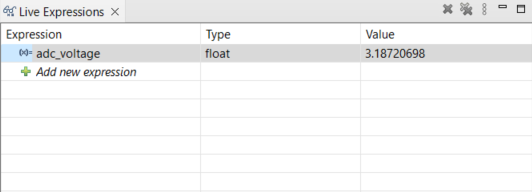
\includegraphics[width=1\linewidth]{fig/KY-013/działanie_ukladu/cieple.png}
\caption{Napięcie po podgrzaniu modułu}
  \label{fig:sub2}
\end{subfigure}
\caption{Porównanie napięć wyjściowych w temperaturze pokojowej oraz po podgrzaniu powietrza źródłem ciepła}
\label{fig:test}
\end{figure}
\begin{figure}[h!]
    \centering
    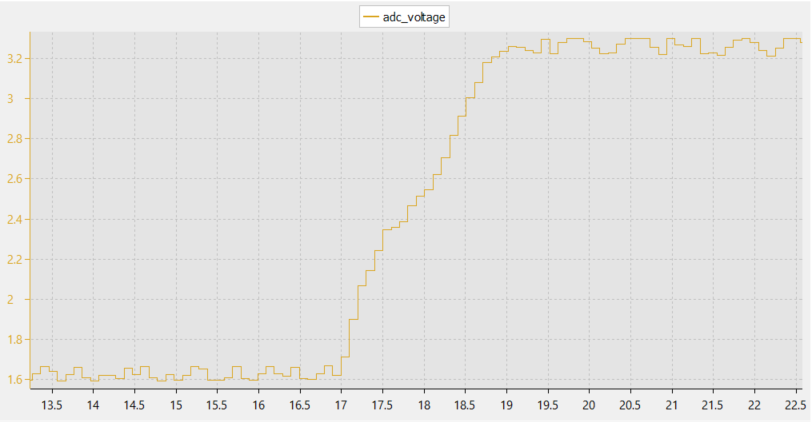
\includegraphics[width=1\textwidth]{fig/KY-013/działanie_ukladu/swv.png}
    \caption{Zmiana napięcia wyjściowego w czasie}
    \label{fig:my_label}
\end{figure}

Rys.6 prezentuje odczyt wartości napięcia wyjściowego w stanie, gdy moduł jest w temperaturze pokojowej, oraz po podgrzaniu powietrza źródłem ciepła w postaci ognia - widoczny jest wzrost z wartości około 1.6V do okolic 3.2V. Zgodnie z zasadą działania, po zwiększeniu się temperatury, spadła rezystancja termistora wbudowanego w moduł.
\newline 

Kod programujący czujnik, wykorzystany do opracowania instrukcji, znajduje się w materiałach dodatkowych zawartych pod koniec rozdziału.
\newline
Film prezentujący działanie układu znajduje się w suplemencie wideo.
\printbibliography[heading=bibintoc]

\end{document}